

%%%  یک نمونه سمینار کارشناسی ارشد، نسخه 0.4
%%%  وحید دامن‌افشان، دانشگاه تبریز،       http://www.damanafshan.ir
%%%  تالار گفتگوی پارسی‌لاتک،       http://forum.parsilatex.com
%%%   آپدیت شده در تیرماه ۹۱


% توجه داشته باشید برای دیدن خروجی کامل شامل نمایه و فهرست مطالب در ویرایشگر Texmaker، ابتدا دو بار 
% کلید F1  را فشار دهید. سپس با استفاده از خط فرمان، به مسیر پوشه جاری رفته و دستور 
% xindy -L persian -C utf8 -M texindy -M page-ranges vahid-seminar.idx
% را در خط فرمان اجرا کنید. سپس دوباره، ۲ بار دیگر کلید F1 را فشار دهید.
% توضیحات مربوط به هر بسته یا دستور را می‌توانید در خط بالای آن ببینید.

\documentclass[12pt,a4paper]{article}
%در ورژن جدید زی‌پرشین برای تایپ متن‌های ریاضی، این سه بسته، حتماً باید فراخوانی شود
\usepackage{amsthm,amssymb,amsmath}
%بسته‌ای برای تنطیم حاشیه‌های بالا، پایین، چپ و راست صفحه
%\usepackage[top=50mm, bottom=50mm, left=50mm, right=50mm]{geometry}

\usepackage{graphicx}
% بسته‌ و دستوراتی برای ایجاد لینک‌های رنگی با امکان جهش 
\usepackage[pagebackref=false,colorlinks,linkcolor=blue,citecolor=magenta]{hyperref}
% چنانچه قصد پرینت گرفتن نوشته خود را دارید، خط بالا را غیرفعال و  از دستور زیر استفاده کنید چون در صورت استفاده از دستور زیر‌‌، 
% لینک‌ها به رنگ سیاه ظاهر خواهند شد و برای پرینت گرفتن، مناسب‌تر است
%\usepackage[pagebackref=false]{hyperref}
% بسته‌ای برای ظاهر شدن «مراجع» و« نمایه» در فهرست مطالب
\usepackage{tocbibind}
% دستورات مربوط به ایجاد نمایه
\usepackage{makeidx}
\makeindex
%%%%%%%%%%%%%%%%%%%%%%%%%%
% فراخوانی بسته زی‌پرشین و دستورات مربوط به نوع فونت‌ها\theoremstyle{theorem}

\usepackage{xepersian}
\settextfont[Scale=1.1]{XB Niloofar}
% وارد کردن دستور بالا الزامی نیست؛ چون در صورت وارد نکردن آن، فونت پیش‌فرض به صورت خودکار، فراخوانی می‌شود.
% چنانچه می‌خواهید که اعداد داخل فرمول‌ها، فارسی باشد، دستور زیر را فعال کنید
%\setdigitfont{Yas}
%%%%%%%%%%%%%%%%%%%%%%%%%%
% تعریف قلم‌های فارسی و انگلیسی برای استفاده در بعضی از قسمت‌های متن
\defpersianfont\titr[Scale=1]{XB Titre}
\defpersianfont\nastaliq[Scale=1.5]{IranNastaliq}
\defpersianfont\traffic[Scale=1]{B Traffic}
% چنانچه فونت B Traffic را ندارید، دستور بالا را غیرفعال کرده و دستور زیر را فعال کنید.
%\defpersianfont\traffic[Scale=1]{XB Niloofar}
%%%%%%%%%%%%%%%%%%%%%%%%%%
%تعریف و نحوه ظاهر شدن عنوان قضیه‌ها، تعریف‌ها، مثال‌ها و ..
%%%%%%%%%%%%%%%%%%%%%%%%%%
% تعریف دستورات جدید برای خلاصه نویسی و راحتی کار در هنگام تایپ فرمول‌های ریاضی
\newcommand{\bR}{\mathbb{R}}
\newcommand{\cB}{\mathcal{B}}
\newcommand{\cO}{\mathcal{O}}
\newcommand{\cG}{\mathcal{G}}
\newcommand{\rM}{\mathrm{M}}
\newcommand{\rC}{\mathrm{C}}
\newcommand{\rV}{\mathrm{V}}
\newcommand{\ls}{\mathrm{LSC}_{+}(X)}
\newcommand{\ce}{\mathrm{C}^{*}(X)}
%%%%%%%%%%%%%%%%%%%%%%%%%%
% تغییر نام کلمه «اثبات» به «برهان»
\renewcommand\proofname{\textbf{برهان}}
\newcommand{\enfootnote}[1]{\footnote{\lr{#1}}}
%%%%%%%%%%%%%%%%%%%%%%%%%%
\begin{document}
% دستوری برای زدن شماره صفحه‌ها به صورت الف، ب، ج و ... (معمولاً در در هر نوشته‌ای، شماره صفحات تا شروع فصل 
% اول آن متن را به صورت الف، ب، ج و ... وارد می‌کنند)
\pagenumbering{harfi}
% دستوری جهت ظاهر نشدن شماره صفحه (فقط در صفحه جاری)
\thispagestyle{empty}
% دستوری برای کم کردن فاصله بین لوگو و لبه بالایی صفحه خروجی
\vspace*{-25mm}
% نحوه درج کردن لوگوی دانشگاه
\centerline{
\includegraphics[height=4cm]{Imgs/logo.png}}

\begin{center}
% دستوری برای کم کردن فاصله بین لوگو و خط پایین آن
\vspace{-3mm}
دانشکده مهندسی کامپیوتر و فن‌آوری اطلاعات
% دستوری برای تعیین فاصله بین دو خط
\\[.2cm]

گروه هوش مصنوعی
\\[1cm]
{\Large 
\textbf{گزارش مطالعاتی اول}
}
\\[.4cm]
\baselineskip=2cm
{\titr
\begin{Huge}
تشخیص پلاک خودروهای ایرانی
\end{Huge}}
\\[1cm]
{\Large {\traffic 
استاد راهنما
}
\\[.7cm]
{\Large \nastaliq دکتر صفا بخش }
\\[.7cm]
{\Large\traffic  پژوهشگر
}}
\\[.6cm]
{\Large \nastaliq احمد اسدی}
\\[.2cm]
 بهار ۱۳۹۶
\end{center}

% دستوری برای رفتن به صفحه جدید
\newpage
% دستوری برای تعیین فاصله بین خطوط (نه دو خط) و تا وقتی که مقدار آن تغییر نکند، فاصله بین خطوط، همین مقدار است
\baselineskip=1cm
% دستوری برای ظاهر شدن فهرست مطالب
\tableofcontents
\newpage
\baselineskip=.75cm
% دستوری برای اختصاص دادن یک عدد به شماره صفحه جاری
%\setcounter{page}{3}
% دستوری برای زدن شماره صفحه‌ها به صورت ۱، ۲، ۳ و ...
\pagenumbering{arabic}

\section{مقدمه}
در این گزارش، مختصری از پژوهش‌های پیشین در حوزه تشخیص خودکار پلاک خودروها را از روی تصاویر ثبت شده، بیان نموده و روش پیشنهادی اولیه را برای انجام این کار، ارائه کرده‌ایم. از آن‌جا که شکل کلی پلاک‌ها در کشورهای مختلف متفاوت است، تولید روش‌های تشخیص پلاک برای خواندن پلاک خودروهای ایران از اهمیت بالایی برخوردار می‌شود.
\\
 تعداد زیادی از پژوهش‌هایی که در زمینه تشخیص پلاک خودروها انجام شده‌اند، با اجرای مراحل زیر موفق به تولید نتایج قابل قبولی شده‌اند:
 \begin{enumerate}
 \item جانمایی \enfootnote{Locating} پلاک در تصویر
 \item جداسازی نویسه‌های پلاک
 \item دسته‌بندی تک‌تک نویسه‌های موجود در پلاک
 \end{enumerate}
در سال‌های گذشته عموما همه مراحل با ارائه روش‌های ابتکاری و استفاده از فیلترهای مختلف انجام می‌شدند اما در سال‌های اخیر استفاده از شبکه‌های عصبی کانولوشنی در پژوهش‌های خارجی به چشم می‌خورد.




\section{جانمایی پلاک در تصویر}
در میان پژوهش‌های داخلی و خارجی، روش‌های متنوع و متعددی برای جانمایی پلاک در تصویر ارائه شده‌اند. در این قسمت به بررسی چند مورد از این پژوهش‌ها می‌پردازیم. از جمله اولین پژوهش‌هایی که در این زمینه مطرح شده است می‌توان به پژوهش لی و همکارانش در سال 1994 \cite{lee1994automatic} اشاره کرد. این پژوهش بر روی پلاک خودروهای کره‌ای انجام شده است. برای مقابله با نویز ناشی از منابع نوری مختلف که در تصاویر موجود است، از یک شبکه عصبی پیش‌رو برای تشخیص رنگ پیکسل‌ها استفاده شده است. ساختار این شبکه عصبی ساده پیش‌رو که با الگوریتم پس‌انتشار خطا آموزش داده شده است، در شکل \ref{fig:colorNN} قابل مشاهده است.

\begin{figure}[h]
\centering
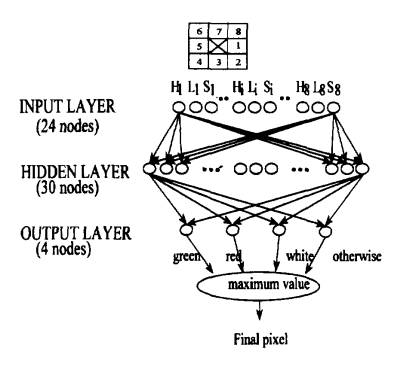
\includegraphics[scale=0.4]{Imgs/colorNN.png}
\caption{ساختار شبکه عصبی مورد استفاده در \cite{lee1994automatic} برای تشخیص رنگ هر پیکسل}
\label{fig:colorNN}
\end{figure}

پس از این‌که رنگ تمام پیکسل‌ها، با استفاده از شبکه عصبی ارائه شده، به یکی از ۴ گروه رنگی تعریف شده، دسته‌بندی شد، هیستوگرام سه رنگ سفید، قرمز و سبز که در پلاک خودروهای کره‌ای مورد استفاده هستند، در دو محور عمودی و افقی رسم می‌شود. این هیستوگرام به عنوان ويژگی‌های تصویر برای یافتن محل پلاک به یک دسته‌بندی کننده داده شده و با استفاده از نتیجه دسته‌بندی کننده، محل دقیق پلاک در تصویر مشخص می‌شود. شکل \ref{fig:hist1} هیستوگرام رسم شده را برای یک تصویر نمونه نمایش می‌دهد.

\begin{figure}[h]
\centering
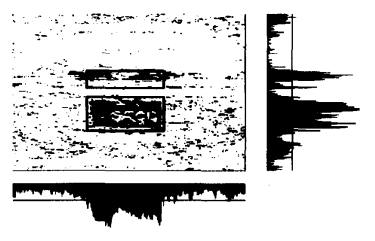
\includegraphics[scale=0.4]{Imgs/hist1.png}
\caption{هیستوگرام رسم‌شده برای یافتن محل پلاک در یک تصویر نمونه در پژوهش \cite{lee1994automatic}}
\label{fig:hist1}
\end{figure}



روش ارائه شده در عین سادگی بسیار زیاد، در شرایط و تصاویر پیچیده عمل‌کرد مناسبی از خود نشان نمی‌دهد. دوان و همکارانش طی دو پژوهش در سال‌های 2004 \cite{duan2004combining} و 2005 \cite{duan2005building} با استفاده از تبدیل هاف و ترکیب آن با روش استخراج کانتورهای فعال\enfootnote{Active Contours} توانستند به دقت 98.8 درصد در تشخیص صحیح محل پلاک خودرو برسند. استفاده از تبدیل هاف به تنهایی کار زمان‌بر و بسیار پرهزینه‌ای است. به همین دلیل در این پژوهش‌ها ابتدا با استخراج پیرامون اشیا با استفاده از کانتورهای فعال و اعمال تبدیل هاف و جستجو بر روی کانتورهای استخراج شده برای پیدا کردن خطوط مستقیم پلاک، زمان و حافظه مورد نیاز برای پردازش و یافتن محل پلاک کاهش چشم‌گیری پیدا کرده است.  شکل \ref{fig:succHF} یک نمونه از تصاویر موجود را در کنار خروجی کانتور فعال آن و  پلاک یافت شده نهایی که با کادر سبز رنگ مشخص شده است، نمایش می‌دهد.


\begin{figure}[h]
\centering
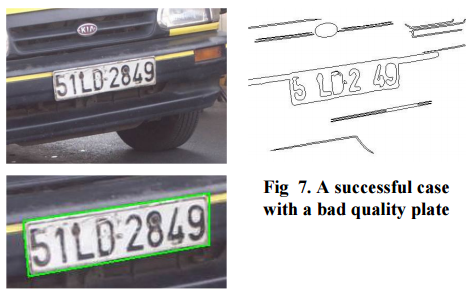
\includegraphics[scale=0.5]{Imgs/succHT.png}
\caption{نتیجه نهایی تشخیص پلاک با استفاده از تبدیل هاف و کانتورهای فعال \cite{duan2004combining}}
\label{fig:succHF}
\end{figure}

در بسیاری از پژوهش‌های دیگر مانند پژوهش‌های
\cite{sanyuan2004car}
،
\cite{sarfraz2003saudi}
،
\cite{zheng2005efficient}
،
\cite{kanayama1991development}
،
\cite{kamat1995efficient}
و
\cite{busch1998feature}
تلاش برای پیدا کردن محل پلاک به اعمال فیلتر لبه‌یاب سوبل\enfootnote{Sobel} و یافتن خطوط عمودی و افقی و بررسی نسبت طول به عرض مستطیل‌های یافت شده و مقایسه آن با نسبت استاندارد طول و عرض پلاک‌ خودروها محدود شده است. در پژوهش \cite{zheng2005efficient} علاوه بر موارد فوق، پس از حذف یال‌های پس‌زمینه و اعمال روش تنها به یال‌های باقی‌مانده، در بین 1165 تصویر، دقت حدود 100٪ حاصل شده است. در این پژوهش ادعا شده زمان پردازش هر تصویر به ابعاد $384 * 288$ پیکسل روی یک کامپیوتر شخصی 47.9 میلی‌ثانیه بوده است.
\\
تمام روش‌های فوق در صورتی که لبه‌های پلاک مخدوش شده یا دچار اعوجاج شده باشند، قابلیت خود را از دست می‌دهند.  روش‌های زیادی برای حل این مشکل از دسته‌بندی ویژگی‌های بافت تصاویر استفاده نموده‌اند. این روش‌ها عموما سعی در استفاده از وجود ارقام و حروف داخل پلاک برای تشخیص محل پلاک دارند. یکی از ساده‌ترین و محبوب‌ترین این روش‌ها اسکن کردن در یک خط مستقیم است. به عنوان مثال پژوهش‌ \cite{xu2005new} یکی از پژوهش‌هایی است که از این تکنیک در سال 2005 استفاده نموده است.
\\
در پژوهش \cite{xu2005new} ابتدا با اعمال فیلتر میانه\enfootnote{Median Filter} به تصویر، تاثیر نویز‌های موجود را کاهش می‌دهند. سپس گرادیان تصویر را در راستای محور افقی محاسبه می‌نمایند. با آستانه‌ای سازی تصویر حاصل، تصویر جدیدی به وجود می‌آید که در آن جهش‌های نقطه‌ای شدید به رنگ سفید و مابقی تصویر به رنگ مشکی نمایش داده شده‌اند. این جهش‌های نقطه‌ای عموما نمایش‌دهنده محل نویسه‌های پلاک هستند. شکل \ref{fig:grad1} تصویر حاصل را روی دو نمونه از تصاویر موجود نمایش می‌دهد. 

\begin{figure}[h]
\centering
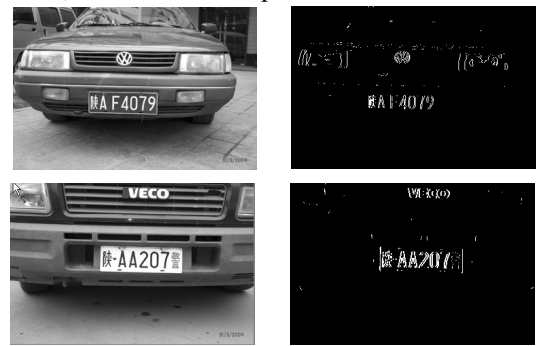
\includegraphics[scale=0.4]{Imgs/grad1.png}
\caption{نتایج آستانه‌ای‌سازی تصویر گرادیان \cite{xu2005new}}
\label{fig:grad1}
\end{figure}

با توجه به این‌ نکته که این پژوهش روی پلاک‌های خودروهای چینی انجام شده است و معمولا روی پلاک‌های خودروهای چینی ۷ نویسه وجود دارد، انتظار داریم در صورتی که خطی افقی را روی تصویر پلاک قرار دهیم، در امتداد خط حداقل  7 نقطه جهش روی تصویر آستانه‌ای شده گرادیان وجود داشته باشد. با اعمال این روش روی تصاویر محل پلاک‌ها با دقت خوبی قابل تشخیص است. میانگین زمان پردازش هر تصویر در این پژوهش 0.36 ثانیه است و دقت نهایی حاصل در آن 96 درصد گزارش شده است.
\\
روش‌های متنوع و متعددی برای استخراج ناحیه پلاک خودروها روی تصاویر ارائه شده‌اند که در این قسمت به بیان تعدادی از این روش‌ها بسنده نمودیم. پژوهش \cite{du2013automatic}  در سال 2013 توسط خانم دو ارائه شده است و در آن یک جمع‌بندی از مزایا و معایب روش‌های مختلف استخراج ناحیه پلاک خودروها از تصاویر، ارائه شده است. این جمع‌بندی در شکل \ref{fig:sumtbl1} ارائه شده است.

\begin{figure}[h]
\centering
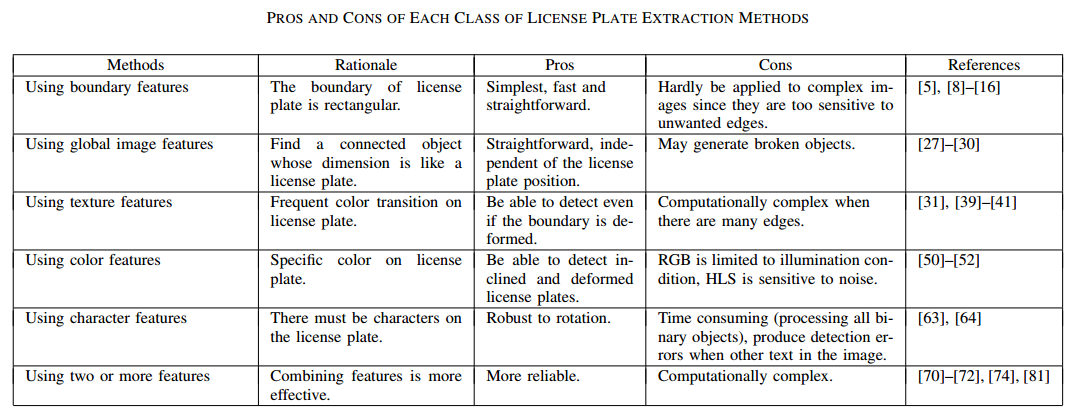
\includegraphics[scale=0.4]{Imgs/sumtbl1.png}
\caption{مزایا و معایب روش‌های مختلف در استخراج ناحیه پلاک \cite{du2013automatic}}
\label{fig:sumtbl1}
\end{figure}


\section{جداسازی نویسه‌های پلاک}
مشابه جانمایی پلاک، روش‌های متنوع و متعددی برای جداسازی نویسه‌ها در پلاک تشخیص‌ داده‌شده، ارائه شده است. در این بخش به بررسی تعدادی از این روش‌ها می‌پردازیم.

\section{دسته‌بندی تک‌تک نویسه‌های موجود در پلاک}


\bibliographystyle{ieeetr-fa}
\bibliography{ref}

\end{document}